%%%%(c)
%%%%(c)  This file is a portion of the source for the textbook
%%%%(c)
%%%%(c)    Abstract Algebra: Theory and Applications
%%%%(c)    Copyright 1997 by Thomas W. Judson
%%%%(c)
%%%%(c)  See the file COPYING.txt for copying conditions
%%%%(c)
%%%%(c)
% Example LaTeX document for GP111 - note % sign indicates a comment
\documentclass[12pt,reqno]{amsart}
\usepackage[top=1.5cm, left=1.5cm,right=1.5cm,bottom=1.5cm]{geometry}
\renewcommand{\baselinestretch}{1.2}
\usepackage{amsmath}
\usepackage{amssymb}
\usepackage{color,hyperref,enumerate,multicol}
\definecolor{darkblue}{rgb}{0.0,0.0,0.3}
\hypersetup{colorlinks,breaklinks,
            linkcolor=darkblue,urlcolor=darkblue,
            anchorcolor=darkblue,citecolor=darkblue}
            
\usepackage{algorithm}
\usepackage{algorithmic}
\pagestyle{empty}
\newcommand{\N}{\ensuremath{\mathbb{N}}}
\newcommand{\Z}{\ensuremath{\mathbb{Z}}}
\newcommand{\R}{\ensuremath{\mathbb{R}}}
\newcommand{\meet}{\ensuremath{\wedge}}
\newcommand{\Meet}{\ensuremath{\bigwedge}}
\newcommand{\join}{\ensuremath{\vee}}
\renewcommand{\emptyset}{\ensuremath{\varnothing}}
\renewcommand{\subset}{\ensuremath{\subsetneq}}
\newcommand{\boldemph}{\emph}
\newcommand{\lcm}{\operatorname{lcm}}

\begin{document}
\thispagestyle{empty}

\noindent \textbf{Math 301} \hskip5cm {\bf Homework 4} \hfill {\bf Fall 2014}
\vskip1cm
\noindent {\bf Chapter 3:}  16, 17, 31, 33, 44, 45, 52. \\  
   Additional suggested exercises: 35, 46, 47, 54.  \\
{\bf Due date:} Friday, 9/26

\medskip

\noindent NOTE: the numbers listed above correspond to the printed version of
the textbook, generated from 2013/08/16 source files.

\medskip

\begin{enumerate}

%% 16 %%%%%%%%%%%%%%%%%%%%%%%%%%%%%%%%%%%%%%%%%%%%%%%%
\item[{\bf 16.}]
Give a specific example of a group $G$ and elements $g, h \in G$ where $(gh)^n \neq g^nh^n$. 
 
\medskip

%% 17 %%%%%%%%%%%%%%%%%%%%%%%%%%%%%%%%%%%%%%%%%%%%%%%%
\item[{\bf 17.}]
Give examples of three different groups with eight elements.  
Why are the groups different? 
 
\medskip

%% 31 %%%%%%%%%%%%%%%%%%%%%%%%%%%%%%%%%%%%%%%%%%%%%%%%
\item[{\bf 31.}]
Show that if $G$ is a finite group of even order, then there is an $a
\in G$ such that $a$ is not the identity and $a^2 = e$.
 
\medskip

%% 33 %%%%%%%%%%%%%%%%%%%%%%%%%%%%%%%%%%%%%%%%%%%%%%%%
\item[{\bf 33.}]
Find all the subgroups of ${\mathbb Z}_3 \times {\mathbb Z}_3$. Use this
information to show that ${\mathbb Z}_3 \times {\mathbb Z}_3$ is not the
same group as ${\mathbb Z}_9$.  (See Example 40
for a short description of the product of groups.)

\medskip

%% 44 %%%%%%%%%%%%%%%%%%%%%%%%%%%%%%%%%%%%%%%%%%%%%%%%
\item[{\bf 44.}]
Prove that the intersection of two subgroups of a group $G$ is also a
subgroup of $G$. 
 
\medskip

%% 45 %%%%%%%%%%%%%%%%%%%%%%%%%%%%%%%%%%%%%%%%%%%%%%%%
\item[{\bf 45.}]
Prove or disprove:  If $H$ and $K$ are subgroups of a group $G$, then
$H \cup K$ is a subgroup of $G$. 

\medskip

%% 52 %%%%%%%%%%%%%%%%%%%%%%%%%%%%%%%%%%%%%%%%%%%%%%%%
\item[{\bf 52.}]
Prove or disprove: Every nontrivial subgroup of an nonabelian group is
nonabelian.

\medskip
\end{enumerate}

\noindent {\bf Additional suggested exercises.}

\begin{enumerate}

\medskip

%% 35 %%%%%%%%%%%%%%%%%%%%%%%%%%%%%%%%%%%%%%%%%%%%%%%%
\item[{\bf 35.}]
Compute the subgroups of the symmetry group of a square.

\medskip

%% 46 %%%%%%%%%%%%%%%%%%%%%%%%%%%%%%%%%%%%%%%%%%%%%%%%
\item[{\bf 46.}]
Prove or disprove: If $H$ and $K$ are subgroups of a group $G$, then
$H K = \{hk : h \in H \text{ and } k \in K \}$ is a subgroup of $G$.
What if $G$ is abelian? 

\medskip

%% 47 %%%%%%%%%%%%%%%%%%%%%%%%%%%%%%%%%%%%%%%%%%%%%%%%
\item[{\bf 47.}]
Let $G$ be a group and $g \in G$. Show that
\[
Z(G) = \{ x \in G : gx = xg \mbox{ for all $g \in G$}
\}\label{centerofagroup} 
\]
is a subgroup of $G$. This subgroup is called the 
\emph{center} of $G$. 
 

\medskip

%% 54 %%%%%%%%%%%%%%%%%%%%%%%%%%%%%%%%%%%%%%%%%%%%%%%%
\item[{\bf 54.}]
Let $H$ be a subgroup of $G$.  If $g \in G$, show that $gHg^{-1} =  \{g^{-1}hg : h\in H\}$ is also a subgroup of $G$.

\end{enumerate}

\end{document}


\item
Find all $x \in {\mathbb Z}$ satisfying each of the following equations.
\begin{multicols}{2}
\begin{enumerate}

\item 
$3x \equiv 2 \pmod{ 7}$

\item
$5x + 1 \equiv 13 \pmod{ 23}$

\item
$5x + 1 \equiv 13 \pmod{ 26}$

\item
$9x \equiv 3 \pmod{ 5}$

\item
$5x \equiv 1 \pmod{ 6}$

\item
$3x \equiv 1 \pmod{ 6}$

\end{enumerate}
\end{multicols}
  

 
 \item   %%%%%%%%%%%%%%%%%%%%%%%%%
Which of the following multiplication tables defined on the set $G =
\{ a, b, c, d \}$ form a group? Support your answer in each case. 
\begin{multicols}{2}
\begin{enumerate}

\item
\[
\begin{array}{c|cccc}
\circ & a & b & c & d \\
\hline
a & a & c & d & a \\
b & b & b & c & d \\
c & c & d & a & b \\
d & d & a & b & c
\end{array}
\]



\item
\[
\begin{array}{c|cccc}
\circ & a & b & c & d \\
\hline
a & a & b & c & d \\
b & b & a & d & c \\
c & c & d & a & b \\
d & d & c & b & a
\end{array}
\]

 
 
\item
\[
\begin{array}{c|cccc}
\circ & a & b & c & d \\
\hline
a & a & b & c & d \\
b & b & c & d & a \\
c & c & d & a & b \\
d & d & a & b & c
\end{array}
\]

\item
\[
\begin{array}{c|cccc}
\circ & a & b & c & d \\
\hline
a & a & b & c & d \\
b & b & a & c & d \\
c & c & b & a & d \\
d & d & d & b & c
\end{array}
\]

\end{enumerate}
\end{multicols}

%% TWJ, 2013/1/2
%% Cayley tables are now in math mode
 
\item   %%%%%%%%%%%%%%%%%%%%%%%%%%%%%%%%%%%
Write out Cayley tables for groups formed by the symmetries of a
rectangle and for $({\mathbb Z}_4, +)$. How many elements are in each
group? Are the groups the same? Why or why not? 
 
 
\item %3
Describe the symmetries of a rhombus and prove that the set of
symmetries forms a group. Give Cayley tables for both the symmetries
of a rectangle and the symmetries of a rhombus. Are the symmetries of
a rectangle and those of a rhombus the same?
 
 
\item %4
Describe the symmetries of a square and prove that the set of
symmetries is a group. Give a Cayley table for the symmetries. How
many ways can the vertices of a square be permuted?  Is each
permutation necessarily a symmetry of the square?  The symmetry group
of the square is denoted by $D_4$.
 
 
\item
Give a multiplication table for the group $U(12)$.
 
 
\item
Let $S = {\mathbb R} \setminus \{ -1 \}$ and define a binary operation on
$S$ by $a \ast b = a + b +ab$. Prove that $(S, \ast)$ is an abelian
group.
 
 
\item
Give an example of two elements $A$ and $B$ in $GL_2({\mathbb R})$ with
$AB \neq BA$.
 
 
\item
Prove that the product of two matrices in $SL_2({\mathbb R})$ has
determinant one.
 
 
\item
Prove that the set of matrices of the form
\[
\begin{pmatrix}
1 & x & y \\
0 & 1 & z \\
0 & 0 & 1
\end{pmatrix}
\]
is a group under matrix multiplication.  This group, known as the
\boldemph{Heisenberg group},\index{Group!Heisenberg} is important in
quantum physics.  Matrix multiplication in the Heisenberg group is
defined by  
\[
\begin{pmatrix}
1 & x & y \\
0 & 1 & z \\
0 & 0 & 1
\end{pmatrix}
\begin{pmatrix}
1 & x' & y' \\
0 & 1 & z' \\
0 & 0 & 1
\end{pmatrix}
=
\begin{pmatrix}
1 & x+x' & y+y'+xz' \\
0 & 1 & z+z' \\
0 & 0 & 1
\end{pmatrix}.
\]
 
 
\item %10
Prove that $\det(AB) = \det(A) \det(B)$ in $GL_2({\mathbb R})$. Use this
result to show that the binary operation in the group $GL_2({\mathbb R})$
is closed; that is, if $A$ and $B$ are in $GL_2({\mathbb R})$, then $AB
\in GL_2({\mathbb R})$.
 
 
\item %11
Let ${\mathbb Z}_2^n = \{ (a_1, a_2, \ldots, a_n) : a_i \in {\mathbb Z}_2
\}$. Define a binary operation on ${\mathbb Z}_2^n$ by
\[
(a_1, a_2, \ldots, a_n)
+
(b_1, b_2, \ldots, b_n)
=
(a_1+b_1, a_2+b_2, \ldots, a_n+b_n).
\]
Prove that ${\mathbb Z}_2^n$ is a group under this operation. This group
is important in algebraic coding theory. 
 
 
\item
Show that ${\mathbb R}^{\ast} = {\mathbb R} \setminus \{0 \}$ is a group
under the operation of multiplication. 
 
 
\item
Given the groups  ${\mathbb R}^{\ast}$ and ${\mathbb Z}$, let $G = {\mathbb
R}^{\ast}  \times {\mathbb Z}$. Define a binary operation $\circ$ on $G$
by $(a,m) \circ (b,n) = (ab, m+n)$. Show that $G$ is a group under
this operation. 
 
 
\item
Prove or disprove that every group containing six elements is abelian.
 
 
\item
Give a specific example of some group $G$ and elements $g, h \in G$
where $(gh)^n \neq g^nh^n$. 
 
 
\item %12
Give an example of three different groups with eight elements.  Why
are the groups different? 
 
 
\item
Show that there are $n!$ permutations of a set containing $n$ items. 
 
 
\item
Show that 
\[
0 + a  \equiv a + 0  \equiv a \pmod{ n }
\]
for all $a \in {\mathbb Z}_n$.
 
 
\item
Prove that there is  a multiplicative identity for the integers modulo
$n$: 
\[
a \cdot  1   \equiv  a \pmod{ n}.
\]
 
 
\item
For each $a \in {\mathbb Z}_n$ find a $b \in {\mathbb Z}_n$ such that
\[
a+b \equiv b+a  \equiv 0 \pmod{ n}.
\]
 
 
\item
Show that addition and multiplication mod $n$ are well defined operations.  That is, show that the operations do not depend on the choice of the representative from the equivalence classes mod $n$.

%% Added exercise.  Suggested by D. Keeler. TWJ 1/10/2014
 
 
\item
Show that addition and multiplication mod $n$ are associative
operations. 
 
 
\item
Show that multiplication distributes over addition modulo $n$:
\[
a  (b  + c)  \equiv a  b + a  c  \pmod{ n}.
\]
 
 
\item
Let $a$ and $b$ be elements in a group $G$.  Prove that $ab^na^{-1} =
(aba^{-1})^n$ for $n \in \mathbb Z$. 
%% Reworded exercise to include $n \in \mathbb Z$. Suggested by Bryce Davis. TWJ 2/10/2012
 
 
\item
Let $U(n)$ be the group of units in ${\mathbb Z}_n$. If $n > 2$, prove that
there is an element $k \in U(n)$ such that $k^2 = 1$ and $k \neq 1$.
 
 
\item
Prove that the inverse of $g _1 g_2 \cdots g_n$ is $g_n^{-1}
g_{n-1}^{-1} \cdots g_1^{-1}$. 
 
 
%% TWJ, 2010/03/31
%% The case $ax = b$ is proved in the text.
%% TWJ, 2011/11/20
%% Changed Theorem to Proposition at the suggestion of G. Tzanakis.
\item
Prove the remainder of Proposition 3.6: if $G$ is a group and $a, b \in G$, then
the equation $xa = b$ has unique solutions in $G$. 
 
%% TWJ, 2010/03/31
%% New Exercise
\item
Prove Theorem 3.8.
 
 
\item
Prove the right and left cancellation laws for a group $G$; that is,
show that in the group $G$, $ba = ca$ implies $b = c$ and $ab = ac$
implies $b = c$ for elements $a, b, c \in G$.  
 
\item
Show that if $a^2 = e$ for all elements $a$ in a group $G$, then $G$ must be abelian. 
%% Reworded exercise. Suggested by Isaac Coombs. TWJ 8/24/2011
 
 
\item
Show that if $G$ is a finite group of even order, then there is an $a
\in G$ such that $a$ is not the identity and $a^2 = e$.
 
 
\item
Let $G$ be a group and suppose that $(ab)^2 = a^2b^2$ for all $a$ and
$b$ in $G$.  Prove that $G$ is an abelian group. 
 
 
\item
Find all the subgroups of ${\mathbb Z}_3 \times {\mathbb Z}_3$. Use this
information to show that ${\mathbb Z}_3 \times {\mathbb Z}_3$ is not the
same group as ${\mathbb Z}_9$.  (See Example 40
for a short description of the product of groups.)
 
 
\item
Find all the subgroups of the symmetry group of an equilateral
triangle. 
 
 
\item
Compute the subgroups of the symmetry group of a square.
 
 
\item
Let $H = \{2^k : k \in {\mathbb Z} \}$. Show that $H$ is a subgroup of
${\mathbb Q}^*$. 
 
 
\item
Let $n = 0, 1, 2, \ldots$ and $n {\mathbb Z} = \{ nk : k \in  {\mathbb Z}
\}$. Prove that $n {\mathbb Z}$ is a subgroup of ${\mathbb Z}$.  Show that
these subgroups are the only subgroups of $\mathbb{Z}$.
 
 
\item
Let ${\mathbb T} = \{ z \in  {\mathbb C}^* : |z| =1 \}$. Prove that ${\mathbb
T}$ is a subgroup of ${\mathbb C}^*$. 
 
 
\item
Let $G$ consist of the $2 \times 2$ matrices of the form
\[
\begin{pmatrix}
\cos \theta & -\sin \theta \\
\sin \theta & \cos \theta
\end{pmatrix}
\]
where $\theta \in {\mathbb R}$. Prove that $G$ is a subgroup of $SL_2(
{\mathbb R})$. 
 
 
\item
Prove that
\[
G =
\{ a + b \sqrt{2} : \mbox{$a, b \in {\mathbb
Q}$ and $a$ and $b$ are not both zero}  \}
\]
is a subgroup of ${\mathbb R}^{\ast}$ under the group operation of
multiplication. 
 
 
\item
Let $G$ be the group of $2 \times 2$ matrices under addition and
\[
H
=
\left\{
\begin{pmatrix}
a & b \\
c & d
\end{pmatrix}
:
a + d = 0
\right\}.
\]
Prove that $H$ is a subgroup of $G$.
 
 
\item
Prove or disprove: $SL_2( {\mathbb Z} )$, the set of $2 \times 2$
matrices with integer entries and determinant one, is a subgroup of
$SL_2( {\mathbb R} )$. 
 
 
\item
List the subgroups of the quaternion group, $Q_8$.
 
 
\item
Prove that the intersection of two subgroups of a group $G$ is also a
subgroup of $G$. 
 
 
\item
Prove or disprove:  If $H$ and $K$ are subgroups of a group $G$, then
$H \cup K$ is a subgroup of $G$. 
 
 
\item
Prove or disprove: If $H$ and $K$ are subgroups of a group $G$, then
$H K = \{hk : h \in H \text{ and } k \in K \}$ is a subgroup of $G$.
What if $G$ is abelian? 
 
 
\item
Let $G$ be a group and $g \in G$. Show that
\[
Z(G) = \{ x \in G : gx = xg \mbox{ for all $g \in G$}
\}\label{centerofagroup} 
\]
is a subgroup of $G$. This subgroup is called the \boldemph{
center}\index{Center!of a group} of $G$. 
 
 
\item
Let $a$ and $b$ be elements of a group $G$. If $a^4b=ba$ and $a^3=e$,
prove that $ab=ba$.
 
 
\item
Let $a$ and $b$ be elements of a group $G$. If $a^4b=ba$ and $a^3=e$,
prove that $ab=ba$.
 
 
\item
Give an example of an infinite group in which every proper subgroup is
finite. 
 
 
\item
If $xy = x^{-1} y^{-1}$ for all $x$ and $y$ in $G$, prove that $G$
must be abelian. 
 
 
%\item
%If $(xy)^2 = xy$ for all $x$ and $y$ in $G$, prove that $G$ must be
%abelian.
%TWJ - 2012/10/21 Exercise deleted since $G$ must also be the trivial group.
 
 
\item
Prove or disprove: Every nontrivial subgroup of an nonabelian group is
nonabelian.
 
 
\item
Let $H$ be a subgroup of $G$ and
\[
C(H) = \{ g \in G : gh = hg \mbox{ for all $h \in H$}  \}.
\]
Prove $C(H)$ is a subgroup of $G$.  This subgroup is called the \boldemph{
centralizer}\index{Centralizer} of $H$ in $G$. 

%Exercise corrected to be the centralizer.  Suggested by Z. Teitler.
%TWJ 12/19/2011

\item
Let $H$ be a subgroup of $G$.  If $g \in G$, show that $gHg^{-1} =  \{g^{-1}hg : h\in H\}$ is also a subgroup of $G$.

%Exercise suggested by R. Beezer
%TWJ - 12/19/2011
%Updated
%TWJ = 2012/10/21
 
\end{enumerate}
}
 
 
\subsection*{Additional Exercises: Detecting Errors}
 
 
{\small
Credit card companies, banks, book publishers, and supermarkets all
take advantage of the properties of integer arithmetic modulo $n$ and
group theory to obtain error detection schemes for the identification
codes that they use. 
\begin{enumerate}
 

%% TWJ, 2010/03/31
%% Fixed figure reference

%% TWJ, 2012/10/21
%% Deleted the word "now" in the description of UPC symbols.  Suggested by R. Beezer.

\item
\textbf{UPC Symbols.}
Universal Product
Code\index{Universal Product Code} (UPC) symbols are found on most
products in grocery and retail stores. The UPC symbol is a 12-digit
code identifying the manufacturer of a product and the product itself
(Figure~\ref{groups_figure_3}). The first 11 digits contain information about the
product; the twelfth digit is used for error detection. If $d_1 d_2
\cdots d_{12}$ is a valid UPC number, then  
\[
3 \cdot d_1 + 1 \cdot d_2 + 3 \cdot d_3 + \cdots + 3 \cdot
d_{11} + 1 \cdot d_{12} \equiv 0 \pmod{10}.
\]
\begin{enumerate}
 
\item
Show that the UPC number  0-50000-30042-6, which appears in
Figure~\ref{groups_figure_3}, is a valid UPC number. 
 
\item
Show that the number 0-50000-30043-6 is not a valid UPC number.
 
\item
Write a  formula to calculate the check digit, $d_{12}$, in the UPC number. 
 
\item
The  UPC error detection scheme can detect most transposition errors; that is, it can determine if two digits have been interchanged.  Show that the transposition error 0-05000-30042-6 is not detected.  Find a transposition error that is detected.  Can you find a general rule for the types of transposition errors that can be detected?
%% Corrected exercise. Suggested by John Watterlond. TWJ 8/24/2011
 
\item
Write a program that will determine whether or not a UPC number is valid. 
 
\end{enumerate}
 
\begin{figure}
\begin{center}
\centerline {
\ifthenelse{\boolean{basic}}
{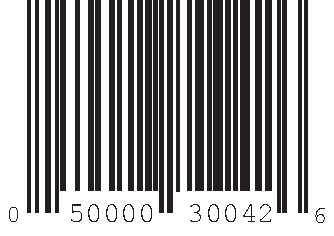
\includegraphics[width=2in]{images/UPCcode.pdf}}{}
\ifthenelse{\boolean{xhtml}}
{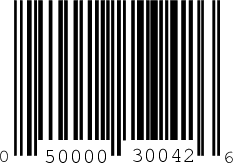
\includegraphics{images/UPCcode.png}}
}
\end{center}
\caption{A UPC code}
\label{groups_figure_3}
\end{figure}

\item
It is often useful to use an inner product notation for this type of error detection scheme; hence, we will use the notion
\[
(d_1, d_2, \ldots, d_k ) \cdot (w_1, w_2, \ldots, w_k ) \equiv 0 \pmod{ n }
\]
to mean
\[
d_1 w_1 +  d_2 w_2 + \cdots +  d_k w_k  \equiv 0  \pmod{ n}.
\]

Suppose that $(d_1, d_2, \ldots, d_k ) \cdot (w_1, w_2, \ldots, w_k ) \equiv 0 \pmod{ n}$ is an error detection scheme for the $k$-digit identification number $d_1 d_2 \cdots d_k$, where $0 \leq d_i < n$.  Prove that all single-digit errors are detected if and only if $\gcd( w_i, n ) = 1$ for  $1 \leq i \leq k$. 

\item
Let $(d_1, d_2, \ldots, d_k ) \cdot (w_1, w_2, \ldots, w_k ) \equiv 0 \pmod{ n}$ be an error detection scheme for the $k$-digit identification number $d_1 d_2 \cdots d_k$, where $0 \leq d_i < n$.  Prove that all transposition errors of two digits $d_i$ and $d_j$ are detected if and only if $\gcd( w_i - w_j, n ) = 1$ for $i$ and  $j$ between 1 and $k$. 

\item
\textbf{ISBN Codes.} 
Every book has an International Standard Book Number\index{International standard book number} (ISBN) code.  This is a 10-digit code indicating the book's publisher and title.  The tenth digit is a check digit satisfying 
\[
(d_1, d_2, \ldots, d_{10} ) \cdot (10, 9, \ldots, 1 )  \equiv 0 \pmod{11}.
\]
One problem is that $d_{10}$ might have to be a 10 to make the inner product zero; in this case, 11 digits would be  needed to make this scheme work.  Therefore, the character X is used for the eleventh digit.  So ISBN 3-540-96035-X is a valid ISBN code. 
\begin{enumerate}
 
 \item
Is ISBN 0-534-91500-0 a valid ISBN code?  What about ISBN 0-534-91700-0 and ISBN 0-534-19500-0? 
 
 \item
Does this method detect all single-digit errors?  What about all transposition errors? 
 
 \item
How many different ISBN codes are there?
 
 \item
Write a computer program that will calculate the check digit for the first nine digits of an ISBN code. 
 
 \item
A publisher has houses in Germany and the United States.  Its German prefix is 3-540.  If its United States prefix will be 0-\textit{abc}, find \textit{abc} such that the rest of the ISBN code will be the same for a book printed in Germany and in the United States. Under the ISBN coding method the first digit identifies the language; German is  3 and English is  0.  The next group of numbers identifies the publisher, and the last group identifies the specific book. 
 
\end{enumerate}
 


}
 
 
 
\subsection*{References and Suggested Readings} % references checked and updated - TWJ 6/22/2010
 
 
{\small
References [2] and [3] show  how group theory can be used in error
detection schemes.  Other sources cover more advanced
topics in group theory. 
\begin{itemize}
 
\item[\textbf{[1]}]  %%Reference updated - TWJ 6/22/2010
Burnside, W. \textit{Theory of Groups of Finite Order}. 2nd ed. Cambridge
University Press, Cambridge, 1911; Dover, New York, 1953.  A classic.  Also available at books.google.com.
 
\item[\textbf{[2]}]
Gallian, J. A. and Winters, S. ``Modular Arithmetic in the
Marketplace,'' \textit{The American Mathematical Monthly} \textbf{
95}(1988): 548--51. 
 
\item[\textbf{[3]}]  %%Reference updated - TWJ 6/22/2010
Gallian, J. A. 
\textit{Contemporary Abstract Algebra}. 7th ed. Brooks/Cole, Belmont, CA, 2009. 
 
\item[\textbf{[4]}]   %%Reference updated - TWJ 6/22/2010
Hall, M. \textit{Theory of Groups}. 2nd ed. American Mathematical Society, Providence, 1959.

 
\item[\textbf{[5]}] %%Reference updated - TWJ 6/22/2010
Kurosh, A. E. \textit{The Theory of Groups}, vols. I and II. American Mathematical Society, Providence, 1979. 
 
 
%%  The following two books are out of print and probably not readily available - TWJ 6/22/2010 

%\item[\textbf{[6]}]  
%MacDonald, I. D. \textit{The Theory of Groups}. Krieger, London, 1988.
% 
%\item[\textbf{[7]}]
%Rose, J. S. \textit{A Course on Group Theory}. Cambridge University
%Press, Cambridge, 1978.
 
 
\item[\textbf{[6]}] %%Reference updated 6/22/2010 - TWJ
Rotman, J. J. \textit{An Introduction to the Theory of
Groups}. 4th ed. Springer, New York, 1995.
 
\end{itemize}
}
 
\sagesection
